%======================================================================
\chapter{Photocatalysis of \texorpdfstring{CO\textsubscript{2}}{CO2}}\label{chap.co2}
\markright{Photocatalysis of \texorpdfstring{CO\textsubscript{2}}{CO2}}
%======================================================================

%======================================================================
\section{Introduction}
%======================================================================

Only 6 years after the photophysical properties of \ce{Re^I} complexes using 2,2'-bipyridine were characterized\autocite{morse1976}, Hawecker, Lehn, and Ziessel showed the effectiveness of the compound for the photocatalytic reduction of \ce{CO2}\autocite{hawecker1983}. Since then, many have shown the efficacy of a wide range of $\alpha$-diimino complexes for the reaction\autocite{hawecker1986, kurz2006, portenkirchner2014} and expansion of the systems to bimetallic complexes with ruthenium and osmium as electron transfer agents has produced a wide range of results\autocite{rossenaar1996, takeda2008, tamaki2013}. The mechanism of reduction has been subject of some debate: while mechanisms have been proposed since Lehn et. al. soon after their original publication\autocite{hawecker1986}, modifications have been submitted routinely over the past decades\autocite{hayashi2003, morris2009, takeda2008, grills2010, agarwal2011, agarwal2012a, agarwal2012b, keith2013}. 

The development of a novel terdentate geometry and the associated increase in photon absorption at lower energies of the catalyst warranted investigation of the \ce{CO2} reduction capabilities, having overcome the criticism of only absorbing high energy photons \autocite{kutal1985}. The terdentate complexes were tested and compared to the bidentate, and to the previously proven catalyst \ce{$\kappa$^2(bipy)Re(CO)3Cl}. 

%======================================================================
\section{Photocatalytic Reactions with New Compounds}
%======================================================================

The photocatalytic cycle is, simply, a photon-induced \gls{ac.mlct}, followed by the extraction of an electron from a sacrificial reductant. This negatively charged radical species sheds the halide anion, opening up a reaction site. Reduction of \ce{CO2} yields any number of \ce{CO}, \ce{H2O}, formate (\ce{HCO2-}), or bicarbonate (\ce{CO3H-}), depending on the mechanistic pathway (see \autoref{scheme.threepath}). Further discussion and a proposal of a new mechanism geometry based on computational and experimental data can be read in \autoref{chap.mech}.

%----------------------------------------------------------------------
\subsection{Conditions}
%----------------------------------------------------------------------

Reaction conditions in use in literature have remained typically unchanged since the original papers. A mixture of \gls{ac.dmf} with either \gls{ac.teoa} or \gls{ac.tea} at a 5:1 ratio is used to make a 1.0 mM solution of catalyst, with `excess' (depending on reference, a 1.1 to 25 molar ratio) electrolyte salt (typically \ce{Et4NX} or \textit{t}-\ce{Bu4NX}, where X = halide from catalyst) added as a stabilizer. Solutions are degassed by bubbling of \ce{CO2}, and a pure \ce{CO2} headspace is left to form over the solution. The reaction of 4~mL of catalyst solution in a 30~mL sealed glass vial is monitored via \gls{ac.gc} analysis of the headspace, using a HP gas chromatograph with a 15~m CARBONPLOT column with 0.320~mm inner diameter and 1.50~$\mu$m film in a 40~$^\circ$C oven. The instrument is fitted with a \gls{ac.tcd}, and, while using He as a carrier gas, is able to resolve \ce{CO} and \ce{CO2} completely.  

%----------------------------------------------------------------------
\subsection{Experimental Results}
%----------------------------------------------------------------------

Both bidentate and terdentate \ce{$\kappa$^n(terpy)Re(CO)_{5-n}X} (n=2, 3) \textbf{2.1} and \textbf{2.2} complexes show no activity for \ce{CO2} reduction. Modification of testing time, light source, product analysis methods, solvent, sacrificial reductant, pH, presence of electrolyte, presence of \ce{H2O}, or variation of anion (X=Cl, Br, OTf, CN) shows no change of this inactivity. Testing of \ce{$\kappa$^2(bipy)Re(CO)3Cl} under the same reaction and testing conditions shows production of approximately 6 mL \ce{CO} from \ce{CO2} (~20\% conversion) in 1 hour of photolysis with visible ($\lambda$~\textgreater ~400~nm) light, verifying the method and isolating the particular catalysts as the ineffective species. 

%======================================================================
\subsection{Rationalization of Results}\label{ss.rationalization}
%======================================================================

The lack of reactivity of the \ce{$\kappa$^2(terpy)Re(CO)3X} motif of complexes contrasting to the activity of the originally published \ce{$\kappa$^2(bipy)Re(CO)3X} indicates significant influence of the ligand on the reaction. Kurz \textit{et al.} demonstrated the requirement for fluorescence for successful catalytic candidates\autocite{kurz2006}. The explanation for this is the requirement for a stable, long-lasting excited state, with lifetime greater than that of the timescale of the electron abstraction from the sacrificial amine. Observed fluorescence demonstrates the lack of non-radiative relaxation pathways, considered to be an analogue for the extended lifetime of the excited state. Sample \textbf{2.2} shows only poor fluorescence (see \autoref{chap.newchem}, \autoref{ss.fluorescence}). While the complex is able to absorb light across the spectrum, and has \gls{ac.homo} to \gls{ac.lumo} transitions with high enough energy\footnote{Electrochemical reduction of \ce{CO2} in similar environments takes 1.7-2.1 V, equivalent to \gls{ac.homo}-\gls{ac.lumo} transitions from 590-750 nm\autocite{grills2014}.} for the catalyzed reduction of \ce{CO2} to \ce{CO}, it appears as if the catalysis is not initiated due to a short excited state lifetime.

Explanation for the lack of \ce{CO} production observed in the attempted photochemical reduction of \ce{CO2} by bidentate sample \textbf{2.1} and others must come from some other area. These samples are quite fluorescent, emission from the powder sample can be seen with the naked eye with simulation by a 405~nm laser pen under ambient light environments. Other substituted bipyridine ligands are known to be active for photocatalytic reduction \autocite{hawecker1986, kurz2006}, thereby suggesting the most likely conflicting feature of the terpyridine ligand to be the pendant arm itself.

\begin{figure}[!htbp]
 \begin{center}
  \includegraphics[clip=true, keepaspectratio, width=80mm]{images/yellowred.eps}
 \end{center}
 \caption[A photograph of aged and fresh catalytic mixture.]{A photograph of fresh (left) and aged (right) catalyst mixtures, showing the change from yellow to red in five days.}
 \label{fig.yellowred}
\end{figure}

Importantly, two clues come from the reaction mixture: under intense visible light in the presence of \ce{CO2} the compound bleaches from bright yellow (see the left vial, \autoref{fig.yellowred}) to a very faint yellow-green. Colour does not return after storage in the dark, bubbling of new \ce{CO2}, or other manipulations. Secondly, a mixture of sacrificial amine, \gls{ac.dmf}, and catalyst \textbf{2.1} in ratios identical to what is required in the reaction mixture changes colour from a yellow to a deep red irreversibly after approximately five days at ambient conditions, as shown in \autoref{fig.yellowred}. 

The most likely cause for the bleaching of the solution is the disassociation of terpyridine ligand from the metal centre. The colours seen in the catalyst are all due to metal-ligand interaction, and the UV-Vis spectrum of free terpyridine in solution is located solely in the UV range ($\lambda$\textsuperscript{max}~$\approx$~285~nm)\autocite{martin1956}. The labilization can be a photoinduced process\autocite{zink2001}. 

\begin{figure}[!htb]
 \begin{center}
  \includegraphics[clip=true, keepaspectratio, width=120mm]{images/yellowreduvvis.eps}
 \end{center}
 \caption[UV-Visible spectra of freshly prepared and aged catalyst mixture.]{UV-Visible spectra of freshly prepared and aged catalyst mixture. DMF, and DMF-TEOA + \ce{Et4NCl} (1 mM) are shown in black and blue, respectively. Fresh catalyst is shown in yellow (1 mM), and green (0.25 mM). Aged catalyst is shown in red (1 mM).}
 \label{fig.reduvvis}
\end{figure}

The UV-visible spectra was obtained for the red compound formed after 5 days of ageing, showing some distinctive modifications (see \autoref{fig.reduvvis}). A peak appears at ca.~560~nm, and the metal to ligand \textit{d}-$\pi^\ast$ peak at 470 nm is reduced. Additionally, the fresh catalyst as a valley in the spectrum at ca. 285~nm, while the aged sample does not; it in fact has increased adsorption at energies above 310~nm. 

\begin{scheme}[tb]
 \begin{center}
  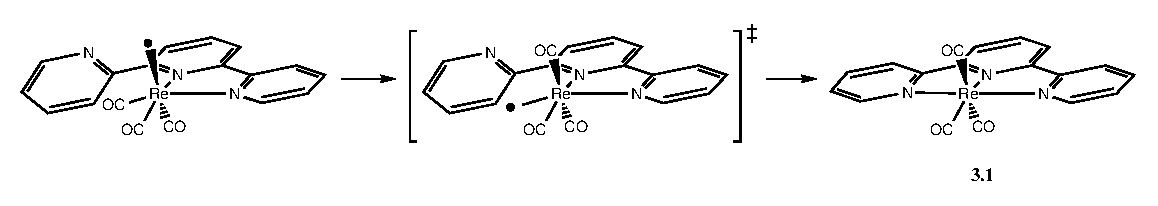
\includegraphics[clip=true, width=\textwidth, keepaspectratio]{images/tricarbscheme.eps}
 \end{center}
\caption[Reorganization from catalytic excimer to form \textbf{3.1}.]{Formation of \textbf{3.1} from catalytic excimer via reorganization of carbonyls and chelation of the pendant arm.}
\label{scheme.tricarbonyl}
\end{scheme}

Other complexes may be formed that deactivate the catalyst, including the formation of a cationic tridentate tricarbonyl complex, seen in \autoref{scheme.tricarbonyl}. This species can be formed by the rearrangement of the carbonyl ligands from the \textit{fac} orientation to a \textit{mer}, migration of one carbonyl to the open site axial to the ligand achieves this reorganization. Once the \textit{mer} species is formed, the open site on the metal centre is oriented towards the pendant arm of the terpyridine ligand, coordination of that group to the metal centre results in compound \textbf{3.1}. The UV-Visible spectra of this species is not isolated, however, \gls{ac.dft} predicted UV-Vis is shown in \autoref{fig.uvvistricarb}, and compared to the experimental red product, these spectra do not correlate. This reorganization may still occur in the reactant solution, but it does not appear to be the primary deactivation pathway.

\begin{figure}[!htbp]
 \begin{center}
  \includegraphics[clip=true, keepaspectratio, width=120mm]{images/tricarbcatuvvisstruct.eps}
 \end{center}
 \caption[Structure and absorption spectra of proposed \ce{[$\kappa$^3-(terpy)-Re(CO)3]+}.]{Computational structure (inset) and predicted UV-Vis absorption spectra of \ce{[$\kappa$^3-(terpy)-Re(CO)3]+} and experimental spectra of the aged catalytic mixture (orange).}
 \label{fig.uvvistricarb}
\end{figure}

Another deactivation product may be the formation of triethanolamine-catalyst adducts\autocite{morimoto2013}. In the presence of DMF, TEOA has been shown to bind to the open site of the excimer via the amine's oxygen atom. This is susceptible to insertion of \ce{CO2} to form a --\ce{OC(O)C}--\ce{CH2CH2N(CH2CH2OH)2} group. \Gls{ac.dft} studies on these two compounds suggest that they may be a coloured species, with predicted UV-Vis showing lower energy absorption than the catalyst itself (a red shift), demonstrated in \autoref{fig.ishitani}. The experimental red mixture UV-Vis spectra is overlaid, showing lack of correlation to the Ishitani compounds.

\begin{figure}[!htbp]
 \begin{center}
  
\includegraphics[clip=true, keepaspectratio, width=120mm]{images/ishitani.eps}
 \end{center}
\caption[Structure and absorption spectra of the catalyst-TEOA complex.]{Computational structure (inset) and \gls{ac.dft} predicted UV-Vis absorption spectra for \textbf{2.1} (blue), the \gls{ac.teoa} complex proposed by Ishitani\autoref{fig.ishitani} (red), and experimental spectra of the aged catalytic mixture (green).}
\label{fig.ishitani}
\end{figure}

Neither the tricarbonyl terdentate nor the Ishitani complexes correlate to the observed spectra in \autoref{fig.reduvvis}. Identification of a compound solely by its spectra is not possible, however, some characteristics could be predicted. It is likely that there is a significant modification of the environment around the metal centre, previous observed electronic transitions that occur at that energy are due to metal \textit{d} to ligand $\pi^\ast$ interactions. Ligand $\pi$~to~$\pi^\ast$ transitions appear at much higher energy, and modification of those interactions could explain the lack of valleys observed in  the UV region (at 285~nm). Further determination of the complex is not possible with the collected data.

Attempts to isolate this red compound were unsuccessful. It appears to be highly soluble in the reaction mixture, not allowing for isolation via solvent extraction.  \Gls{ac.dmf} and \gls{ac.teoa} are high-boiling point solvents, any attempts to remove solvent via distillation (even at low pressure) required temperatures approaching the thermolysis temperature for synthesis of the terdentate compounds. Further investigation is required to isolate the product.

%======================================================================
\section{Conclusions}
%======================================================================

Experimental data shows the inactivity of these catalysts for photoreduction of \ce{CO2} under a range of experimental conditions. These same conditions show conversion using \ce{$\kappa$^2(bipy)Re(CO)3Cl} as the photoreductant, signifying the validity of experimental setup. The inactivity may be due to formation of inactive side-products or ligand labilization (for the case of bidentate catalyst) or due to the short excited state lifetime of the terdentate catalyst. 

Catalyst mixtures appear to form a new compound after ageing. Although isolation was not achieved, this red product was investigated via UV-Vis spectroscopy, the spectra was compared to \gls{ac.dft} calculated spectra for two potential deactivation products. The spectra do not align, suggesting that the red product is some as of yet unknown compound. 
